\begin{figure*}
\centering
\begin{subfigure}[h]{0.5\textwidth}
\caption{}
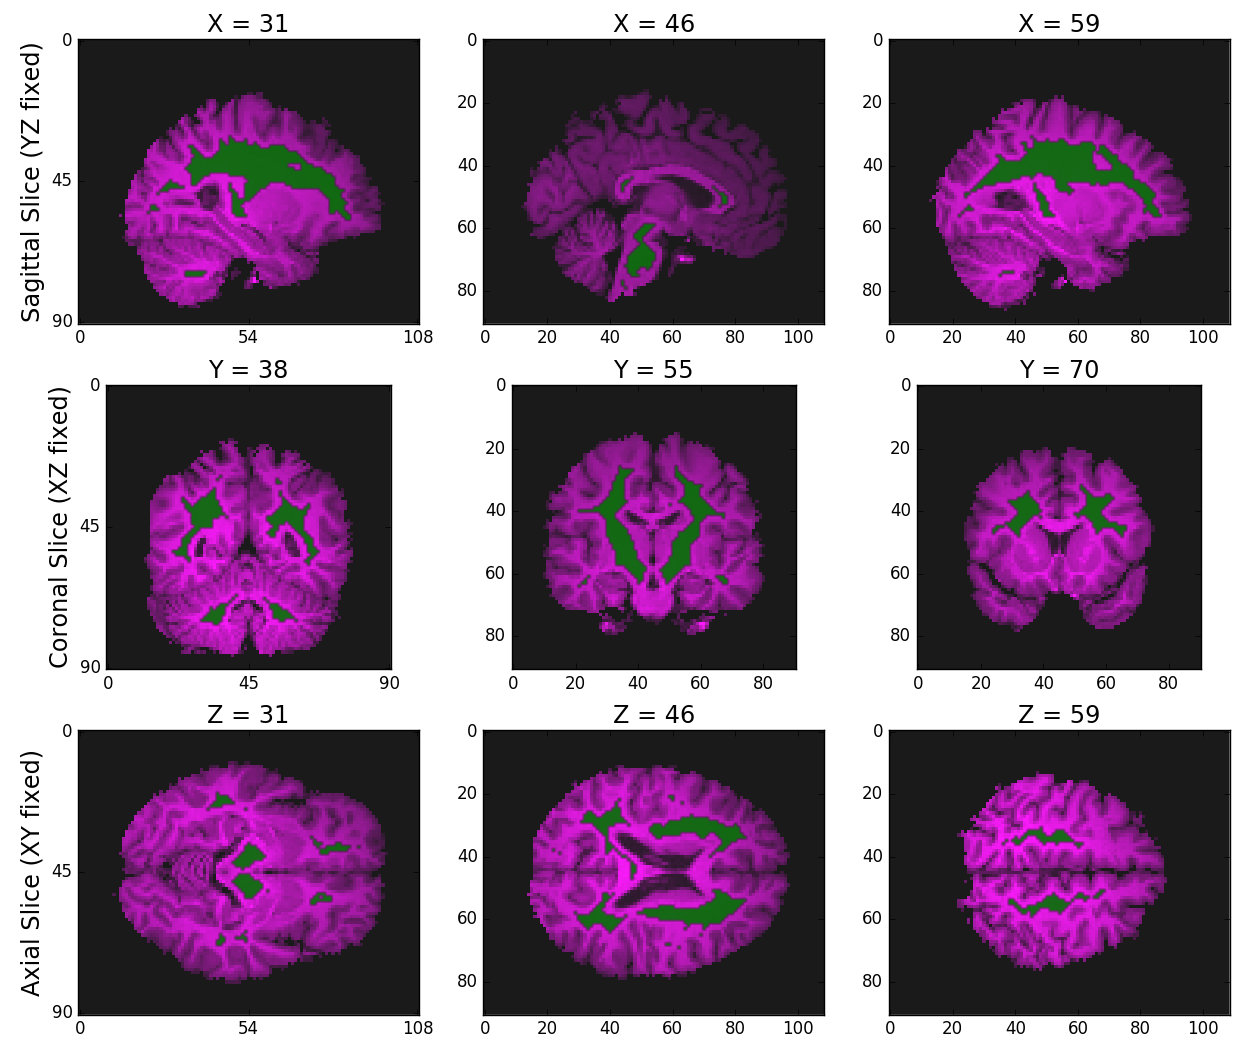
\includegraphics[width=\textwidth]{./qa_figs/fig_fmri_nuis_eroded_wm.png}
\label{fig:er_wmm}
\end{subfigure}
\begin{subfigure}[h]{0.45\textwidth}
\caption{}
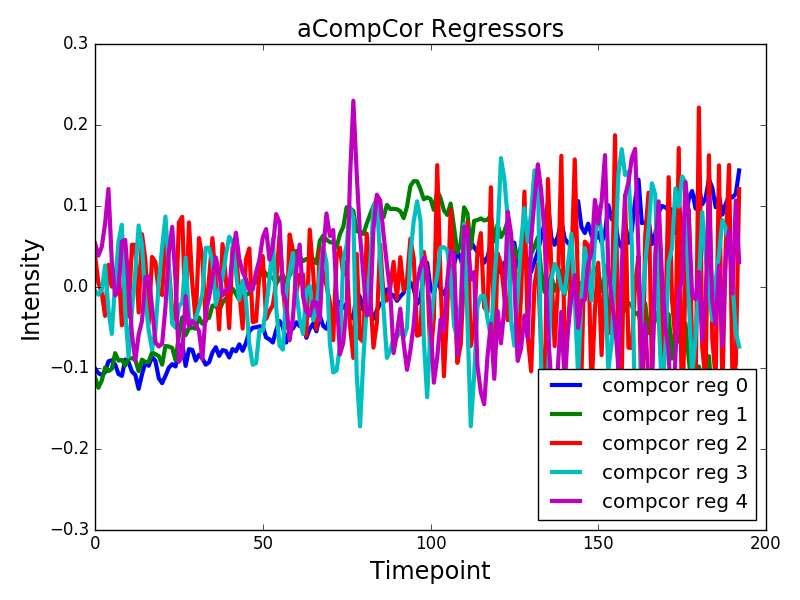
\includegraphics[width=\textwidth]{./qa_figs/fig_fmri_nuis_compcor_reg.png}
\label{fig:ccreg}
\end{subfigure}
\begin{subfigure}[h]{0.45\textwidth}
\caption{}
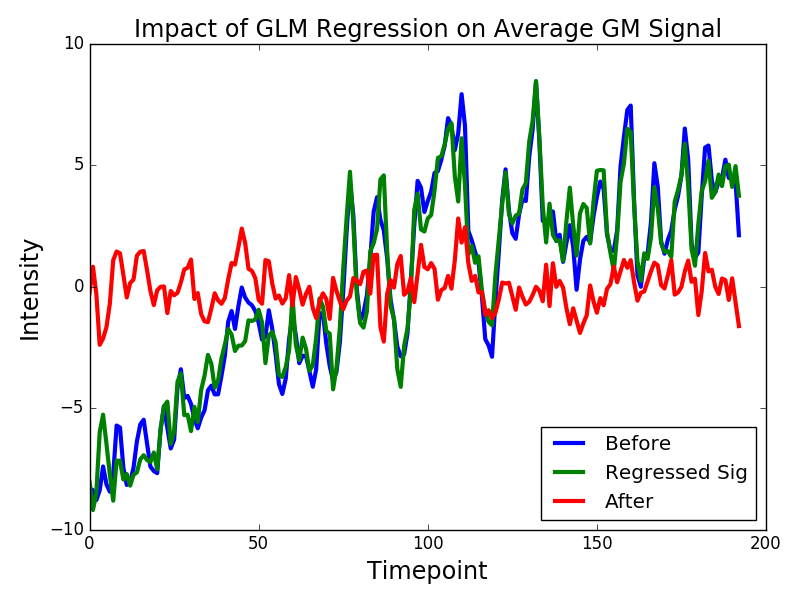
\includegraphics[width=\textwidth]{./qa_figs/fig_fmri_nuis_glm_signal_cmp.png}
\label{fig:glm}
\end{subfigure}
\begin{subfigure}[h]{0.45\textwidth}
\caption{}
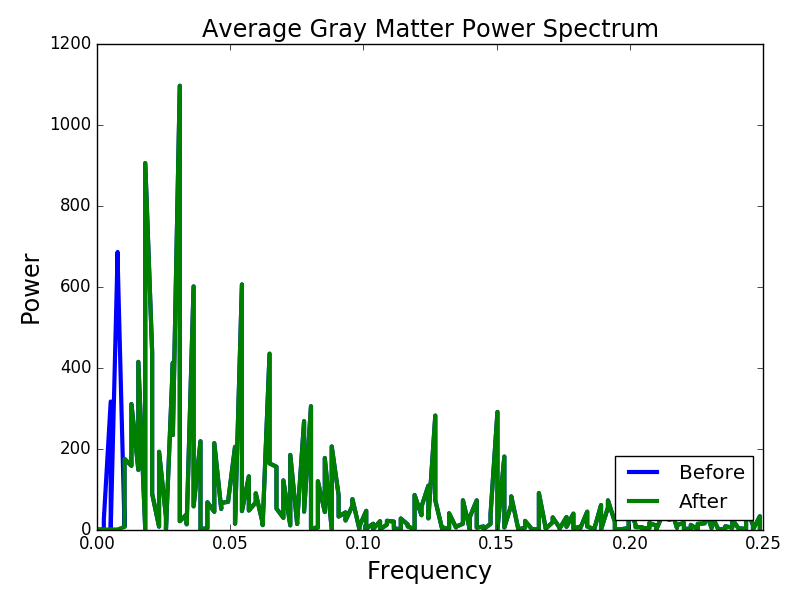
\includegraphics[width=\textwidth]{./qa_figs/fig_fmri_nuis_power.png}
\label{fig:power}
\end{subfigure}
\caption{\textbf{\ndmgf~Nuisance Correction QA}.  \ndmgf~produces QA figures focusing on the nuisance regressors. 
(A) The white matter, gray matter, cerebro-spinal fluid, and eroded white matter mask used to compute aCompcorr. 
(b) For the General Linear Model, the time varying regressors estimated from the eroded white matter and cerebro-spinal timemseries by aCompCor.
(c) 
%the regressors estimated by the Friston 24 parameter model, and t
The average gray matter signal before and after regression. 
(d) 
For frequency filtering, we show the average gray matter signal before and after frequency filtering, and the average gray matter power spectrum before and after filtering.}
\label{fig:fmri_nuis}
\end{figure*}